\documentclass{article}
\usepackage{graphicx} % Required for inserting images

\title{DevOps24-groupK\\
\large Course Code: BSDSESM1KU}
\author{GitGurus}
\date{Spring 2024}

% \usepackage{graphicx} % Required for inserting images
% \usepackage{amsmath}
% \usepackage{hyperref}
\usepackage{listings}
\lstset
{
    basicstyle=\footnotesize,
    numbers=left,
    stepnumber=1,
    showstringspaces=false,
    tabsize=1,
    breaklines=true,
    breakatwhitespace=false,
}

\usepackage[utf8]{inputenc}
\usepackage[T1]{fontenc}
\usepackage[english]{babel}
\usepackage{minted}
% \usepackage[a4paper, bottom=3cm, top=3cm, left=2.5cm, right=2.5cm]{geometry}
\usepackage[linewidth=1pt]{mdframed}
\usepackage{ebproof}
\usepackage{amsmath}
% \usepackage{fourier}
\usepackage{booktabs}
% \usepackage{inconsolata}
\usepackage{float}
\usepackage{lastpage}
\usepackage{graphicx}
\usepackage{titling}
\usepackage{fancyhdr}
\usepackage[dvipsnames]{xcolor}
\usepackage[hidelinks]{hyperref}

\renewcommand{\baselinestretch}{1.2} % Line spacing
% \setlength{\parindent}{0em} % Paragraph indent
% \setlength{\parskip}{0.75em} % Paragraph vertical spacing

% \colorlet{LightGray}{Gray!7!}

% % global minted styles
% \setminted{bgcolor=LightGray, breaklines, frame=single, linenos, fontsize=\small, numbersep=8pt}

% % minted remove red squares around "erroneus" code
% \AtBeginEnvironment{minted}{%
%   \renewcommand{\fcolorbox}[4][]{#4}}

% % minted line number style
% \renewcommand{\theFancyVerbLine}{{\scriptsize \arabic{FancyVerbLine}}}
\begin{document}

\maketitle

\begin{table}[H]
    \centering
    \begin{tabular}{c|c}
    Andreas Guldborg Hansen & aguh@itu \\
    Andreas Severin Hauch Trøstrup & atro@itu.dk \\
    Frederik Petersen & frepe@itu.dk \\
    Mads Aqqalu Roager & mroa@itu.dk \\
    Silke Holme Bonnen & ssbo@itu.dk
    \end{tabular}
\end{table}

\newpage
\tableofcontents

\newpage


\section{Systems' perspective}
\subsection{Design and architecture}
An overview of the architecture of our MiniTwit application can be found in figure \ref{fig:architecture}. 
The entire system runs on DigitalOcean, with the exception of our monitoring and logging that runs on New Relic.
In DigitalOcean, we have 3 primary nodes running. A swarm manager, and two workers. These 3 nodes are a part of a docker swarm network that runs the minitwit web app and minitwit simulator API containers as docker services.
The workers and manager also run a New Relic agent that collects logs and system monitoring information, and send it to new relic.
The manager node runs a Nginx reverse proxy, that handles https encryption, and load balancing between the workers.
Lastly, in DigitalOcean we also have a managed database running, that acts as the database for the application.
What the diagram below does not show is that the swarm manager also has a container running the web app and the simulator API. The reason why this is not shown on the diagram is because the Nginx reverse proxy has been set to only forward requests to worker 1 and 2. 
That means that the web app and the simulator api in the swarm manager will never be used. 


\begin{figure}[H]
    \centering
    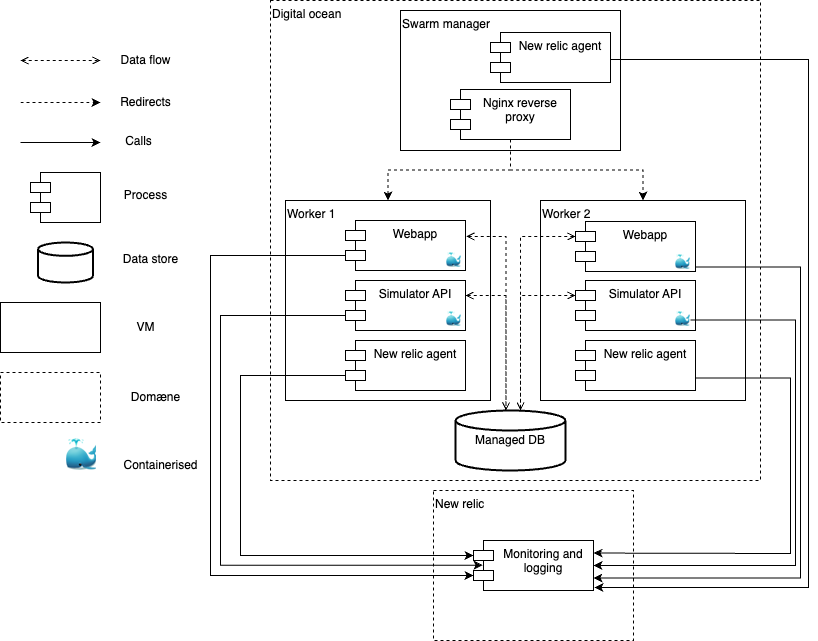
\includegraphics[width=\textwidth]{images/devops-overview.png}
    \caption{The figure shows a diagram of the architecture of minitwit}
    \label{fig:architecture}
\end{figure}

\subsection{Dependencies}
\todo{Describe and illustrate: all dependencies of your ITU-MiniTwit systems on all levels of abstraction and development stages. That is, list and briefly describe all technologies and tools you applied and depend on.
}


DigitialOcean is the only critical dependency for keeping the application running. That is the 3 VM's and the database. 

We do not show further dependecies... 

\begin{figure}[H]
    \centering
    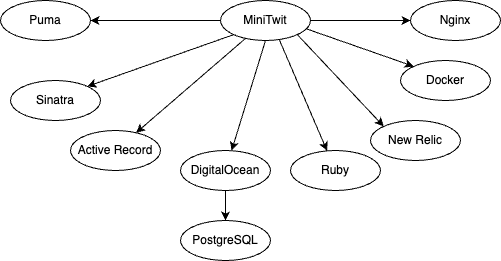
\includegraphics[width=0.8\textwidth]{images/dependency-graph-prod.png}
    \caption{Production dependency graph.}
    \label{fig:dep-prod}
\end{figure}

\subsection{Interactions of subsystems}
\todo{For example, via an illustrative UML Sequence diagram that shows the flow of information through your system from user request in the browser, over all subsystems, hitting the database, and a response that is returned to the user.
Similarly, another illustrative sequence diagram that shows how requests from the simulator traverse your system.
}
\begin{figure}[H]
    \centering
    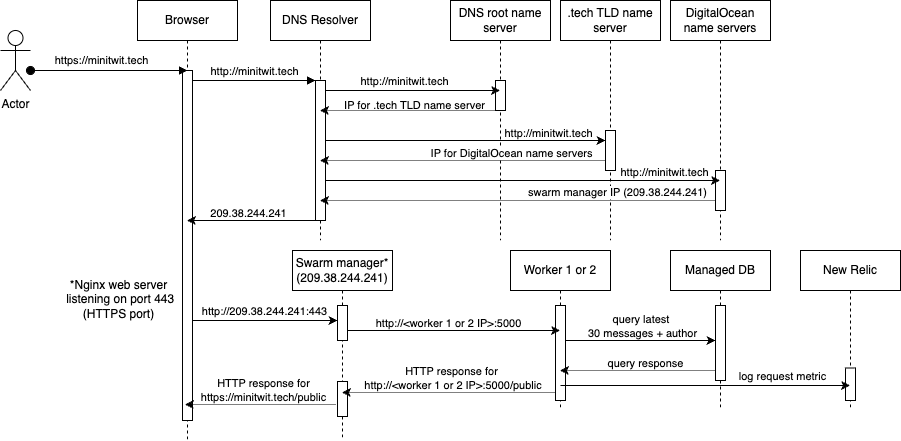
\includegraphics[width=\textwidth]{images/devops-sequence.png}
    \caption{A sequence diagram describing the process of calling "minitwit.tech/public"}
    \label{fig:sequence}
\end{figure}


\begin{figure}[H]
    \centering
    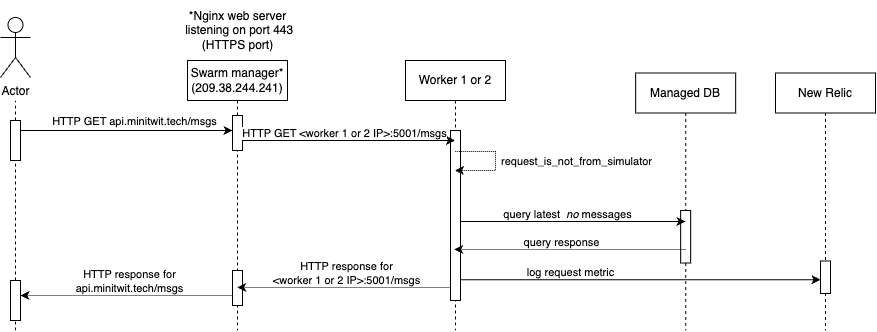
\includegraphics[width=\textwidth]{images/api-sequence.png}
    \caption{A sequence diagram describing the process of calling "api.minitwit.tech/msgs"}
    \label{fig:sequence_api}
\end{figure}


\subsection{Current state}
\todo{Describe the current state of your systems, for example using results of static analysis and quality assessments.}

\section{Process' perspective}
\todo{This perspective should clarify how code or other artifacts come from idea into the running system and everything that happens on the way.
In particular, the following descriptions should be included:}


\subsection{CI/CD chain}
\todo{A complete description of stages and tools included in the CI/CD chains, including deployment and release of your systems. }

\subsubsection{Deployment workflows}
Our deployment workflows runs in GitHub LSP

\subsubsection{Report workflows}
To ensure our report in our repository is always up to date, we utilise a built-in synchronization between Overleaf and GitHub. Once changes are made that a group member wish to save, one click from within Overleaf synchronizes the contents to a separate repository in our GitHub organisation, which triggers two Github Actions workflows:
\begin{enumerate}
    \item A workflow from within this report repository that notifies our main repository of any changes made to our report repository.
    \item A workflow from within the main repository that is called by the previously mentioned workflow, which triggers a git submodule update and commits it to the repository.
\end{enumerate}

\subsection{Monitoring \& Logging}
\todo{How do you monitor your systems and what precisely do you monitor?}
Both monitoring and logging of this project is done using New Relic.
\begin{figure}[h]
    \centering
    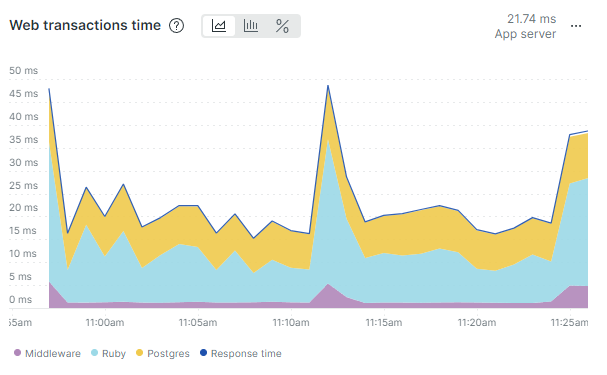
\includegraphics[width=\textwidth]{images/new-relic-transactions.png}
    \caption{The newrelic graph depicting web transaction times by application layer}
    \label{fig:transaction-times}
\end{figure}
% Afsnit done lets go
% det ser faktisk lækkert ud i latex

\todo{What do you log in your systems and how do you aggregate logs?}
% NewRelic er begge dele

\subsection{Security}
\todo{Brief results of the security assessment and brief description of how did you harden the security of your system based on the analysis}

\subsection{Scaling and upgrading}
\todo{Applied strategy for scaling and upgrades}

\subsection{Use of AI tools}
\todo{
In case you have used AI-assistants during your project briefly explain which system(s) you used during the project and reflect how it supported/hindered your process.
}

In the beginning of the project, not all team members were familiar with the programming language Ruby. In order to get familiar, some of us had the Github Copilot extension enabled, allowing us to participate on a similar level as those who were more familiar with the language.\\

In the review process, ChatGPT has been used as a tool to interpret changes made by other members, by prompting ChatGPT to help understand the effects and consequences of the changes.\\

\section{Lessons learned perspective}
\todo{Describe the biggest issues, how you solved them, and which are major lessons learned with regards to: evolution and refactoring,
operation, and
maintenance 
of your ITU-MiniTwit systems. Link back to respective commit messages, issues, tickets, etc. to illustrate these. Also reflect and describe what was the "DevOps" style of your work. For example, what did you do differently to previous development projects and how did it work?}

\subsection{Evolution and refactoring}

\subsection{Operation}

\subsection{Maintenance}

\end{document}


